% MECHANISM-BASED EMULATION
Dynamic simulators can be emulated in a purely statistics-based manner, e.g.\ by conditioning a Gaussian process prior on the experimental design.
Mechanism-based approaches try to enhance the emulation through an appropriate incorporation of the available physical understanding \cite{Hydro:Reichert2011,Hydro:Albert2012,Hydro:Machac2016:b}.
In particular, the solution of a simplified problem is incorporated into the prior and subsequently corrected so as to emulate the full simulator.
An application of this approach to the Adliswil watershed can be found in \cite{Hydro:Machac2016:a}.
\par % PCA+PCE
We pursue an alternative strategy.
First, the model output dimensionality is reduced through principal component analysis.
Then, sparse polynomial chaos expansions are computed for the main components as functions of the uncertain inputs.
Last, the obtained expansions are combined in order to obtain a surrogate model for the full time series of the outflow.

\subsection{Computational model}
% ORIGINAL MODEL
The SWMM implementation of the catchment predicts a complete time series of the outflow at the wastewater treatment plant throughout the precipitation event.
Provided that one inputs the rainfall intensity over the duration of the experiment, the model only acts as a function of the uncertain input parameters listed in \cref{tab:Hydro:Parameters}.
We gather the unknown model input parameters in a vector \(\bm{x} = (x_1,\ldots,x_\dimParam)^\top\) with \(\dimParam = 8\).
Similarly we proceed for the rainfall data \(\bm{d} = (d_0,\ldots,d_\dimData)^\top\) with \(\dimData = 600\).
For \(i=0,\ldots,\dimData\) we have introduced \(d_i = I(t_i)\) for the observed rainfall intensities at the measurement time instances \(t_i\).
\par % MODEL OUTPUT
The numerical model predicts the vector \(\tilde{\bm{y}} = (\tilde{y}_0,\ldots,\tilde{y}_\dimData)^\top\)
whose entries are the outflows \(\tilde{y}_i = \tilde{Q}(t_i)\) at the times \(t_i\).
All in all, \(\tilde{\bm{y}} = \mathcal{M}(\bm{x},\bm{d})\) reflects the structure of the hydrological simulations.
Since we only consider a single precipitation event and disregard errors in the rainfall data,
we absorb the dependence on the rainfall into the definition of the forward model \(\mathcal{M}_{\bm{d}}\) by
\begin{equation} \label{eq:Hydro:ForwardModel}
  \tilde{\bm{y}} = \mathcal{M}_{\bm{d}}(\bm{x}).
\end{equation}
\par % PROBABILISTIC INTERPRETATION
We now switch to a probabilistic formulation,
where the inputs are assumed to be independent and \([\underline{x}_i,\overline{x}_i]\)-valued random variables \(X_i\)
with uniform distributions \(X_i \sim \mathcal{U}(x_i \cond \underline{x}_i,\overline{x}_i)\) for \(i=1,\ldots,\dimParam\).
The random vector \(\bm{X} = (X_1,\ldots,X_\dimParam)^\top\) is then distributed according to
\begin{equation} \label{eq:Hydro:InputRV}
  \bm{X} \sim \prod\limits_{i=1}^\dimParam \mathcal{U}(x_i \cond \underline{x}_i,\overline{x}_i).
\end{equation}
This distribution represents some kind of input uncertainty.
When the model \(\mathcal{M}_{\bm{d}}\) is applied to the random inputs \(\bm{X}\),
the output uncertainty is described by the \(\mathds{R}^{\dimData+1}\)-valued random response vector
\begin{equation} \label{eq:Hydro:OutputRV}
  \tilde{\bm{Y}} = \mathcal{M}_{\bm{d}}(\bm{X}).
\end{equation}
\par % TRAINING RUNS
As already mentioned before, the original implementation of this simulator is only available to us through \(K = 2048\) training runs in total.
We cannot execute it for arbitrary values of the inputs.
Yet we have access to realizations \(\bm{x}^{(k)}\) of the input variables in \cref{eq:Hydro:InputRV} for \(k=1,\ldots,K\)
and the corresponding realizations \(\tilde{\bm{y}}^{(k)} = \mathcal{M}_{\bm{d}}(\bm{x}^{(k)})\) of \cref{eq:Hydro:OutputRV}.
The inputs were obtained by Latin hypercube sampling \cite{MCMC:MacKay1979} in two chunks of \(1024\) samples each.
Altogether they constitute the experimental design \(\mathcal{X} = (\bm{x}^{(1)},\ldots,\bm{x}^{(K)})\).
Moreover, the responses are collected into the data matrix
\begin{equation} \label{eq:Hydro:DataMatrix}
  \mathcal{Y} = \begin{pmatrix}
                  \tilde{\bm{y}}^{{(1)}^\top} \\
                  \tilde{\bm{y}}^{{(2)}^\top} \\
                  \vdots \\
                  \tilde{\bm{y}}^{{(K)}^\top} \\
                \end{pmatrix}
              = \begin{pmatrix}
                  \tilde{y}_0^{(1)} & \tilde{y}_1^{(1)} & \ldots & \tilde{y}_\dimData^{(1)} \\
                  \tilde{y}_0^{(2)} & \tilde{y}_1^{(2)} & \ldots & \tilde{y}_\dimData^{(2)} \\
                  \vdots            & \vdots            & \ddots & \vdots \\
                  \tilde{y}_0^{(K)} & \tilde{y}_1^{(K)} & \ldots & \tilde{y}_\dimData^{(K)} \\
                \end{pmatrix}.
\end{equation}
\par % BLACK-BOX PERSPECTIVE
With that said, we have to embrace a black-box perspective on the present problem.
The information contained in the training runs is used in the computation of a surrogate simulator,
i.e.\ a metamodeling problem with \(\dimParam = 8\) inputs, \(\dimData + 1 = 601\) outputs and \(K = 2048\) training runs is posed.
The problem is solved with a multivariate extension of the polynomial chaos--based methods described in \cref{sec:Uncertainty:SurrogateModeling,sec:Uncertainty:LeastSquares}.

\subsection{Principal components}
% BASIS EXPANSION
Note that a preliminary discussion of the multivariate case was already provided in \cref{sec:Uncertainty:MultivariateOutput}.
The coordinates of the model output with respect to a certain reference system, e.g.\ the canonical basis, can be considered individually.
In our case, this would require to handle about six hundred different metamodels at the same time.
That is inconvenient and involves a high degree of redundancy, i.e.\ the simulation outputs at contiguous times are highly correlated.
\par % PRINCIPAL COMPONENTS
To find a remedy one can choose a basis that is qualified for purposes of dimension reduction and data compression.
Here we use \emph{principal component analysis} (PCA) \cite{Statistics:Dunteman1989,Statistics:Jackson1991,Statistics:Jolliffe2002} to that end.
While this technique is mainly used for compressing big real-word data sets with many features,
it can be similarly used for reducing the model output in the context of computer simulations \cite{PCE:Sudret2011:Proc,PCE:Sudret2013:Proc}.
We start by discussing the population PCA for a random vector,
which is just the discrete variant of the \emph{Karhunen--Lo\`{e}ve} (KL) \emph{expansion} of a stochastic process \cite{Probability:Loeve1977}.
Afterwards the empirical sample PCA is recalled.
\par % RANDOM VECTOR
Consider the random vector \(\tilde{\bm{Y}}\) with mean \(\bm{\mu}_{\tilde{\bm{Y}}} = \mathds{E}[\tilde{\bm{Y}}]\) and covariance matrix
\(\bm{\Sigma}_{\tilde{\bm{Y}}} = \mathrm{Cov}[\tilde{\bm{Y}}] = \mathds{E}[(\tilde{\bm{Y}}-\bm{\mu}_{\tilde{\bm{Y}}})(\tilde{\bm{Y}}-\bm{\mu}_{\tilde{\bm{Y}}})^\top]\).
% EIGENVECTORS
Since \(\bm{\Sigma}_{\tilde{\bm{Y}}}\) is symmetric and positive definite,
one can find linearly independent eigenvectors \(\bm{\phi}_i\) with positive eigenvalues \(\lambda_i > 0\) for \(i=0,\ldots,\dimData\).
The characteristic vectors and values satisfy
\begin{equation} \label{eq:Hydro:Eigenequation}
  \bm{\Sigma}_{\tilde{\bm{Y}}} \bm{\phi}_i = \lambda_i \bm{\phi}_i.
\end{equation}
Eigenvectors corresponding to distinct eigenvalues are orthogonal anyway, while they can be always chosen as such for degenerate eigenvalues.
We assume that the eigenvalues are arranged in decreasing order \(\lambda_0 \geq \lambda_1 \geq \ldots \geq \lambda_\dimData\)
and that eigenvectors are normalized such that \(\bm{\phi}_i^\top \bm{\phi}_j = \delta_{ij}\) for \(i,j=0,\ldots,\dimData\).
Leaving degeneracy aside, this way the eigenvectors are uniquely defined up to a multiplication by \(-1\).
\par % MATRIX DIAGONALIZATION/EIGENDECOMPOSITION
The set of eigenvectors constitutes an orthonormal basis of \(\mathds{R}^{\dimData+1} = \mathrm{span}(\{\bm{\phi}_i\}_{i=0}^\dimData)\).
One can define the orthogonal matrix \(\bm{\Phi} = (\bm{\phi}_0,\bm{\phi}_1,\ldots,\bm{\phi}_\dimData)\)
with \(\bm{\Phi}^\top \bm{\Phi} = \bm{\Phi} \bm{\Phi}^\top = \bm{I}\).
It diagonalizes the covariance matrix by
\begin{equation} \label{eq:Hydro:Diagonaliztaion}
  \bm{\Phi}^\top \bm{\Sigma}_{\tilde{\bm{Y}}} \bm{\Phi}
  = \bm{\Lambda} = \begin{pmatrix}
                     \lambda_0 & 0 & \ldots & 0 \\
                     0 & \lambda_1 & \ldots & 0 \\
                     \vdots & \vdots & \ddots & \vdots \\
                     0 & 0 & \ldots & \lambda_\dimData \\
                   \end{pmatrix}.
\end{equation}
Vice versa, one obtains the spectral eigendecomposition of the covariance matrix
\(\bm{\Sigma}_{\tilde{\bm{Y}}} = \bm{\Phi} \bm{\Lambda} \bm{\Phi}^\top = \sum_{i=0}^\dimData \lambda_i \bm{\phi}_i \bm{\phi}_i^\top\).
% RANDOM VECTOR LINEAR TRANSFORMATION
Now consider the orthogonal transformation
\begin{equation} \label{eq:Hydro:LinearTransformation}
  \tilde{\bm{Z}} = \bm{\Phi}^\top (\tilde{\bm{Y}} - \bm{\mu}_{\tilde{\bm{Y}}}).
\end{equation}
The linearly transformed random vector has mean zero \(\mathds{E}[\tilde{\bm{Z}}] = \bm{0}\)
and the diagonal covariance matrix \(\mathrm{Cov}[\tilde{\bm{Z}}] = \mathds{E}[\tilde{\bm{Z}} \tilde{\bm{Z}}^\top] = \bm{\Lambda}\), i.e.\ it has been centered and decorrelated.
Independence is not necessarily implied thereby, though, the special case involving Gaussianity forms an exception.
The back-transformation reads
\begin{equation} \label{eq:Hydro:BackTransformation}
  \tilde{\bm{Y}} = \bm{\mu}_{\tilde{\bm{Y}}} + \bm{\Phi} \tilde{\bm{Z}} = \bm{\mu}_{\tilde{\bm{Y}}} + \sum\limits_{i=0}^\dimData \tilde{Z}_i \bm{\phi}_i.
\end{equation}
This is the discrete KL expansion of the random vector \(\tilde{\bm{Y}}\).
The random variables \(\tilde{Z}_i = \bm{\phi}_i^\top (\tilde{\bm{Y}}-\bm{\mu}_{\tilde{\bm{Y}}})\) for \(i=0,\ldots,\dimData\) are called the \emph{principal components}.
\par % TOTAL VARIANCE
Define the \emph{total variance} of \(\tilde{\bm{Y}}\) as the sum \(\sum_{i=0}^\dimData \mathrm{Var}[\tilde{Y}_i]\) of the individual variances of \(\tilde{Y}_i\).
The orthogonal transformation preserves the total variance in the sense that
\begin{equation} \label{eq:Hydro:TotalVariance}
  \sum_{i=0}^\dimData \mathrm{Var}[\tilde{Y}_i] = \operatorname{tr}(\bm{\Sigma}_{\tilde{\bm{Y}}})
  = \operatorname{tr}(\bm{\Lambda}) = \sum_{i=0}^\dimData \mathrm{Var}[\tilde{Z}_i] = \sum_{i=0}^\dimData \lambda_i.
\end{equation}
This follows from the invariance of the trace under cyclic permutations.
% OPTIMALITY/COMPACTION
The KL expansion is optimal with respect to compaction of the total variance.
Consider keeping only the first \(\dimData^\prime + 1\leq \dimData + 1\) terms in
\begin{equation} \label{eq:Hydro:TruncatedKLE}
  \tilde{\bm{Y}} \approx \bm{\mu}_{\tilde{\bm{Y}}} + \sum\limits_{i=0}^{\dimData^\prime} \tilde{Z}_i \bm{\phi}_i.
\end{equation}
This is the expansion that contains most of the total variance with \(\dimData^\prime + 1\) terms.
The number of terms is often chosen such that at least a predetermined fraction
\(\sum_{i=0}^{\dimData^\prime} \lambda_i / \sum_{i=0}^\dimData \lambda_i\) of the total variance is explained.
\par % EMPIRICAL SAMPLE PCA
The sample PCA functions in exactly the same way for independent realizations as the population PCA does for random vectors.
Instead of the exact mean \(\bm{\mu}_{\tilde{\bm{Y}}} = \mathds{E}[\tilde{\bm{Y}}]\) and covariance matrix \(\bm{\Sigma}_{\tilde{\bm{Y}}} = \mathrm{Cov}[\tilde{\bm{Y}}]\),
one considers their empirical estimates for the sample \(\mathcal{Y} = (\tilde{\bm{y}}^{(1)},\ldots,\tilde{\bm{y}}^{(K)})^\top\) of realizations from \(\tilde{\bm{Y}}\).
They are given as
\begin{equation} \label{eq:Hydro:EmpiricalMoments}
  \overline{\bm{\mu}}_{\tilde{\bm{Y}}} = \frac{1}{K} \sum\limits_{k=1}^K \tilde{\bm{y}}^{(k)}, \quad
  \overline{\bm{\Sigma}}_{\tilde{\bm{Y}}}
  = \frac{1}{K-1} \sum\limits_{k=1}^K (\tilde{\bm{y}}^{(k)}-\overline{\bm{\mu}}_{\tilde{\bm{Y}}})(\tilde{\bm{y}}^{(k)}-\overline{\bm{\mu}}_{\tilde{\bm{Y}}})^\top.
\end{equation}
For \(i=0,\ldots,\dimData\) the eigenvectors \(\overline{\bm{\phi}}_i\) and eigenvalues \(\overline{\lambda}_i\) of the empirical covariance
fulfill \(\overline{\bm{\Sigma}}_{\tilde{\bm{Y}}} \overline{\bm{\phi}}_i = \overline{\lambda}_i \overline{\bm{\phi}}_i\).
The eigenvalues are arranged in the descending order \(\overline{\lambda}_0 \geq \overline{\lambda}_1 \geq \ldots \geq \overline{\lambda}_\dimData\).
\par % DATA COMPRESSION
Then one finds the smallest \(\dimData^\prime \leq \dimData\) for which the proportion \(\sum_{i=0}^{\dimData^\prime} \overline{\lambda}_i / \sum_{i=0}^\dimData \overline{\lambda}_i\)
of the total empirical variance is larger or at least equal than a prespecified threshold.
The matrix \(\overline{\bm{\Phi}}_{\dimData^\prime} = (\overline{\bm{\phi}}_0,\overline{\bm{\phi}}_1,\ldots,\overline{\bm{\phi}}_{\dimData^\prime})\) is composed
and for \(k=1,\ldots,K\) one defines
\begin{equation} \label{eq:Hydro:CompressedRepresentation}
  \tilde{\bm{z}}^{(k)} = \overline{\bm{\Phi}}_{\dimData^\prime}^\top (\tilde{\bm{y}}^{(k)} - \overline{\bm{\mu}}_{\tilde{\bm{Y}}}).
\end{equation}
This is the reduced PCA representation of \(\tilde{\bm{y}}^{(k)}\) in terms of the empirical principal components
\(\tilde{z}_i^{(k)} = \overline{\bm{\phi}}_i^\top (\tilde{\bm{y}}^{(k)}-\overline{\bm{\mu}}_{\tilde{\bm{Y}}})\) for \(i=0,\ldots,\dimData^\prime\).
The data set is compressed while retaining most of the total variation by
\begin{equation} \label{eq:Hydro:CompressedMatrix}
  \mathcal{Z} = \begin{pmatrix}
                  \tilde{\bm{z}}^{{(1)}^\top} \\
                  \tilde{\bm{z}}^{{(2)}^\top} \\
                  \vdots \\
                  \tilde{\bm{z}}^{{(K)}^\top} \\
                \end{pmatrix}
              = \begin{pmatrix}
                  \tilde{z}_0^{(1)} & \tilde{z}_1^{(1)} & \ldots & \tilde{z}_{\dimData^\prime}^{(1)} \\
                  \tilde{z}_0^{(2)} & \tilde{z}_1^{(2)} & \ldots & \tilde{z}_{\dimData^\prime}^{(2)} \\
                  \vdots            & \vdots            & \ddots & \vdots \\
                  \tilde{z}_0^{(K)} & \tilde{z}_1^{(K)} & \ldots & \tilde{z}_{\dimData^\prime}^{(K)} \\
                \end{pmatrix}.
\end{equation}
The compression of the data is still lossy, but one can reconstruct the originally observed samples for \(k=1,\ldots,K\) approximately as
\begin{equation} \label{eq:Hydro:ApproximateReconstruction}
  \tilde{\bm{y}}^{(k)} \approx \overline{\bm{\mu}}_{\tilde{\bm{Y}}} + \overline{\bm{\Phi}}_{\dimData^\prime} \tilde{\bm{z}}^{(k)}
  = \overline{\bm{\mu}}_{\tilde{\bm{Y}}} + \sum\limits_{i=0}^{\dimData^\prime} \tilde{z}_i^{(k)} \overline{\bm{\phi}}_i.
\end{equation}

\subsection{Sparse expansion}
% OUTPUT PCA
Now we perform PCA to our sample of SWMM simulator responses \(\mathcal{Y} = (\tilde{\bm{y}}^{(1)},\ldots,\tilde{\bm{y}}^{(K)})^\top\).
Using \(\dimData^\prime + 1 = 9\) principal components captures \(\unit[99]{\%}\) of the total variance of the signal.
Hundred realizations contained in the compressed data set \(\mathcal{Z} = (\tilde{\bm{z}}^{(1)},\ldots,\tilde{\bm{z}}^{(K)})^\top\)
are visualized in the parallel coordinate plot in \cref{fig:Hydro:Data:Compression}.
These are the empirical principal components of the sample of training runs that were already shown in \cref{fig:Hydro:Data:Outflow}.
It can be seen that the main components are centered around zero and ordered according to their individual contribution to the total variance.
\par % POLYNOMIAL EXPANSION
With the underlying experimental design \(\mathcal{X}\) and the reduced output data \(\mathcal{Z}\),
PCEs of the population principal components \(\tilde{z}_i(\bm{X})\) are computed separately for \(i=0,\ldots,\dimData^\prime\).
Normalized multivariate Legendre polynomials \(\{\basis_{\bm{\alpha}}(\bm{X})\}_{\bm{\alpha} \in \mathcal{A}_p}\) in the random inputs constitute the expansion basis for all PCEs.
The total degree \(\lVert \bm{\alpha} \rVert_1 = \sum_{i=1}^\dimParam \lvert \alpha_i \rvert \leq p\) is limited to at most \(p=10\).
Only terms with \(\bm{\alpha} \in \mathcal{A}_p = \left\{ \bm{\beta} \in \mathds{N}^\dimParam \colon \lVert \bm{\beta} \rVert_1 \leq p \right\}\) are then kept in the PCEs
\begin{equation} \label{eq:Hydro:PrincipalComponentPCE}
  \tilde{z}_i(\bm{X}) \approx \sum\limits_{\bm{\alpha} \in \mathcal{A}_p} \hat{a}_{i,\bm{\alpha}} \basis_{\bm{\alpha}}(\bm{X}).
\end{equation}
\par % LEAST ANGLE REGRESSION
We use \emph{least angle regression} (LAR) \cite{Statistics:Vidaurre2013,Statistics:Zhang2014} in order to compute the coefficients
\(\{\hat{a}_{i,\bm{\alpha}}\}_{\bm{\alpha} \in \mathcal{A}_p}\) for each expansion with \(i=0,\ldots,\dimData^\prime\).
LAR is a powerful technique that promotes sparsity in the PCE coefficient vectors.
Regressors are penalized such a way that only the most dominant ones are retained in the expansion.
This allows us to mitigate the curse of dimensionality discussed in \cref{sec:Uncertainty:CurseOfDimensionality} to some degree.
The algorithm has been proven very efficient in the context of metamodeling based on polynomial chaos \cite{PCE:Blatman2011}.
We use our own inhouse implementation of LAR \cite{Computing:Uqlab2015:Manual09104}.
\par % LEAVE-ONE-OUT ERRORS
Cross validation is used to assess the generalization performance of the sparse PCEs.
The normalized leave-one-out errors for expansions with \(K=1024\) and \(K=2048\) are reported in \cref{tab:Hydro:PCE:Errors}.
As expected, the PCE with the richer experimental design generalizes better than the one with the poorer design for which the error is approximately twice as high.
One can observe the general trend that the accuracy of the approximation decays with the order of the principal components.
% EXPANSION SPARSITY
As it turns out, the hydrological model is indeed approximately sparse in the polynomial basis used.
Only a small fraction of the total number of regressors is retained in each of the nine expansions.
% TABLE: LEAVE-ONE-OUT ERRORS
\begin{table}[htbp]
  \caption[Normalized leave-one-out errors]{Normalized leave-one-out errors.}
  \label{tab:Hydro:PCE:Errors}
  \centering
  \resizebox{\linewidth}{!}{
  \begin{tabular}{cccccccccc}
    \toprule
    \(K\) & \(\tilde{z}_0\) & \(\tilde{z}_1\) & \(\tilde{z}_2\) & \(\tilde{z}_3\) & \(\tilde{z}_4\) & \(\tilde{z}_5\) & \(\tilde{z}_6\) & \(\tilde{z}_7\) & \(\tilde{z}_8\) \\
    \midrule
    \(1024\) & \(2.58 \times 10^{-5}\) & \(1.42 \times 10^{-4}\) & \(3.94 \times 10^{-4}\) & \(2.22 \times 10^{-4}\)
             & \(3.37 \times 10^{-3}\) & \(2.70 \times 10^{-3}\) & \(7.35 \times 10^{-3}\) & \(7.37 \times 10^{-3}\) & \(1.11 \times 10^{-2}\) \\
    \(2048\) & \(1.49 \times 10^{-5}\) & \(6.87 \times 10^{-5}\) & \(1.73 \times 10^{-4}\) & \(1.06 \times 10^{-4}\)
             & \(1.41 \times 10^{-3}\) & \(1.23 \times 10^{-3}\) & \(2.56 \times 10^{-3}\) & \(2.97 \times 10^{-3}\) & \(3.16 \times 10^{-3}\) \\
    \bottomrule
  \end{tabular}
  }
\end{table}
\par % FINAL SURROGATE
After the computation of a PCE for each principal component in \(\tilde{\bm{z}}(\bm{X}) = (\tilde{z}_0(\bm{X}),\ldots,\tilde{z}_{\dimData^\prime}(\bm{X}))^\top\),
the random vector containing the model outputs is approximately represented as
\begin{equation} \label{eq:Hydro:VectorOutputPCE}
  \tilde{\bm{Y}} \approx \hat{\mathcal{M}}_p(\bm{X}) = \overline{\bm{\mu}}_{\tilde{\bm{Y}}} + \sum\limits_{i=0}^{\dimData^\prime} \tilde{z}_i(\bm{X}) \overline{\bm{\phi}}_i.
\end{equation}
This expansion is henceforth used as a metamodel of the model output
\(\tilde{\bm{y}} \approx \hat{\mathcal{M}}_p(\bm{x}) = \overline{\bm{\mu}}_{\tilde{\bm{Y}}} + \sum_{i=0}^{\dimData^\prime} \tilde{z}_i(\bm{x}) \overline{\bm{\phi}}_i\)
at arbitrary input values \(\bm{x} \in \mathcal{D}_{\bm{x}}\).
This is justified due to the mean-square convergence of the underlying PCEs.
% PREDICTION ACCURACY
In \cref{fig:Hydro:PCE:Accuracy} the simulated and emulated outflows are shown for three different input values in the experimental design.
It is ascertained that the obtained metamodel is sufficiently accurate for parameter calibration purposes.
% FIGURES: COMPRESSED DATA & PREDICTION ACCURACY
\begin{figure}[htbp]
  \begin{minipage}[b]{\HYDROsubWidth}
    \centering
    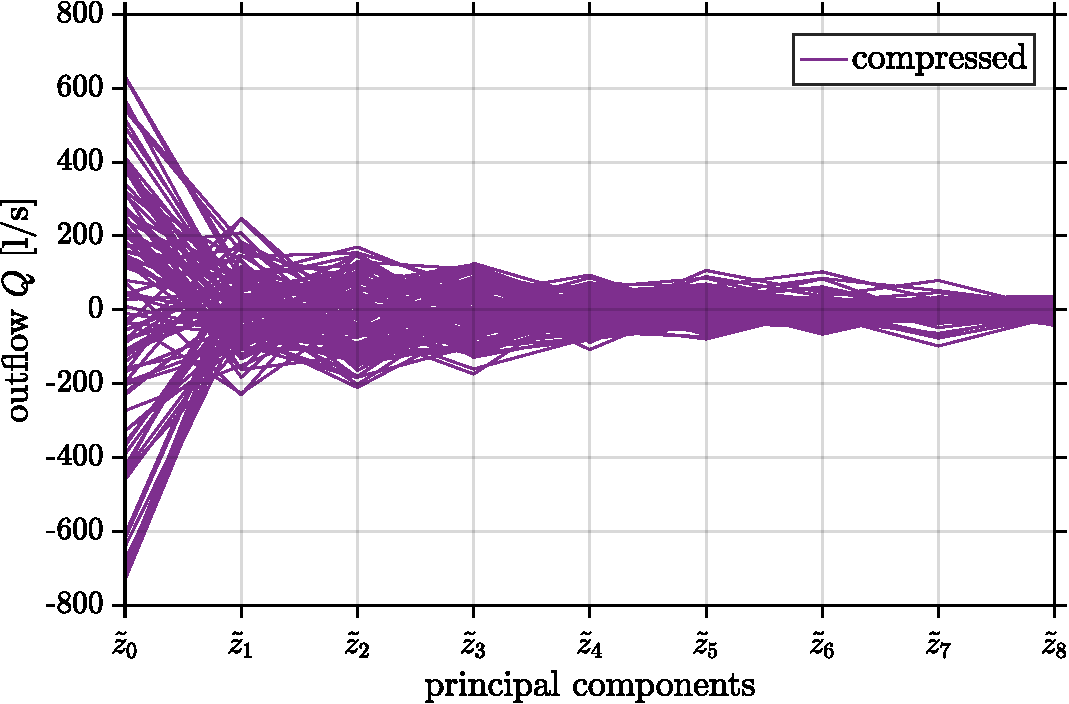
\includegraphics[height=\HYDROfigHeight]{fig_Hydro_Data_Compression}
    \caption[Principal component analysis]{Principal component analysis.}
    \label{fig:Hydro:Data:Compression}
  \end{minipage}%
  \hfill%
  \begin{minipage}[b]{\HYDROsubWidth}
    \centering
    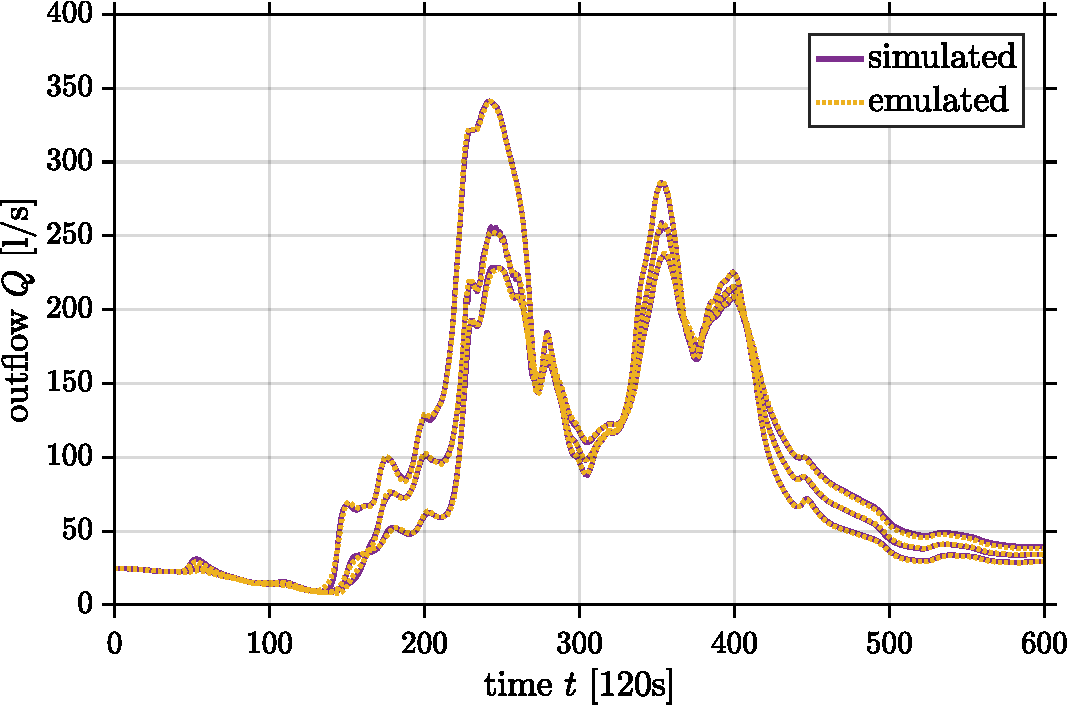
\includegraphics[height=\HYDROfigHeight]{fig_Hydro_PCE_Accuracy}
    \caption[Final metamodel predictions]{Final metamodel predictions.}
    \label{fig:Hydro:PCE:Accuracy}
  \end{minipage}%
\end{figure}